\documentclass[FrontPage]{grattan}
% Comments are deployed by the % sign; everything after % is ignored by the compiler.
% Please do not put comments before \documentclass as these are reserved for TeX directives.
% add_to_dictionary: SSBs? peri-operative Djerriwarrh specialty comorbidity comorbidities accreditors metadata analytical Benchmarking funders cannulation Healthcare GPs unmanageably sequelae intensivists  post-operative pre-operative longtable CHADx HACs DRGs PREMs PROMs Specialty POMR specialties CT Peri-op Post-op Pre-op Peri thromboembolism Clostridium difficile unicompartment Bertillon PICQ Movember Novartis POMR

% add_to_dictionary: POMR
% add_to_dictionary: AIHW

\addbibresource{bib/Grattan-Master-Bibliography.bib}
\addbibresource{bib/health.bib}

\usepackage{longtable}

% release: true

\MONTH{November}
\YEAR{2017}


\author{Stephen Duckett and Christine Jorm}
\title{Strengthening safety statistics: how to make hospital safety data more useful}
\hypersetup{pdfauthor={Stephen Duckett and Christine Jorm and Lucille Danks and Danielle Romanes and Jessy Wu and Naveen Tenneti}}

% add_author_to_recommended_citation_at: Christine Jorm 2

\GrattanReportNumber{2017-11}

\acknowledgements{%
This report was written by Stephen Duckett, Program Director, Christine Jorm, Honorary Fellow, and Lucille Danks, Associate, from the Health Program at Grattan Institute. Danielle Romanes, Jessy Wu and Naveen Tenneti provided extensive research assistance and made substantial contributions to the report.

We would like to thank numerous people from the health policy community including Michael Daly, Deniza Mazevska and Grattan Institute’s Health Program Reference Group for their helpful comments.

The opinions in this report are those of the authors and do not necessarily represent the views of Grattan Institute's founding members, affiliates, individual board members, reference group members or reviewers.
Any remaining errors or omissions are the responsibility of the authors.

Grattan Institute is an independent think-tank focused on Australian public policy.
Our work is independent, practical and rigorous.
We aim to improve policy outcomes by engaging with both decision-makers and the community.

For further information on the Institute's programs, or to join our mailing list, please go to: \textcolor{blue}{\url{http://www.grattan.edu.au/}}.

{\footnotesize
This report may be cited as:
Duckett, S., Jorm, C., and Danks, L\@. (2017). \emph{\mytitle}. Grattan Institute.

ISBN: 978-0-9876121-8-2

All material published or otherwise created by Grattan Institute is licensed under a Creative Commons Attribution-NonCommercial-ShareAlike 3.0 Unported License\par
}
}




\begin{document}


\begin{overview}
Safety scandals in Australian hospitals are depressingly frequent.
They stimulate special reports and an immediate flurry of action. The tragedy is that these safety incidents occur despite reporting, governance and oversight mechanisms that -- if they were working properly -- might have helped to detect the aberrant clinical care.

Lots of information is collected about hospital safety in Australia, but not all of it is shared with the right people. 

Hospital boards are often blissfully ignorant of the safety of care being provided in their hospital. More than 70 per cent of board members in one Victorian survey reported implausibly that quality of care in their hospital was above average; none thought they were below average, and only 3 per cent admitted that they did not really know how their health service compared. But there is a lot of data already collected that could help board members to make an accurate assessment of how safe is the hospital for which they are ultimately responsible.


Australia’s hospitals will be safer if we make data about hospital safety as usable and useful as possible. Hospital boards and management teams – the people responsible for the quality of care in the hospital – need to know what is going on, using all the available data.

This report looks at data on patient outcomes: routine data, clinical quality registry data, death audit data, incident reporting and investigation data, patient-reported experience measures, and patient-reported outcome measures. 

A first step in improving hospital safety in Australia is to better use the information that is already collected, and to put it in the hands of people who can apply it. This report reviews different sources of information about safety of hospital care. It provides background to a series of Grattan Institute reports which will examine hospital safety in more depth.

Our examination reveals many instances where the data could and should be more accurate, relevant, accessible and understandable. Data registries need to share information more widely, they need to capture a greater proportion of the care given, and they need to get data back to clinicians more quickly. States and private hospitals need to give more information to clinicians, including routine data and patient-experience data. The data needs to be clear and detailed, so clinical teams can see how they are performing compared with their peers, and how they can improve. 

Sometimes the information is locked away so only the people who contributed the data can see it – and often then only after a long lag. Some data sets don’t contain enough information. For instance, the narrow remit of the anaesthetic death audit hampers efforts to improve peri-operative care. Some data is not made available quickly enough – old results are of little use to doctors and hospital managers. 

This report makes specific recommendations for each data set, and two overarching recommendations: that the links between data sets should be stronger, and that data should be presented more clearly.

The data we have is an extremely valuable resource. Better use needs to be made of it by governments making it more accurate, relevant, accessible, and understandable.
\end{overview}

%\hyphenpenalty1000
\newcommand*{\rowHeight}{-0.5ex}%\linespread{0.925}
\onecolumn\vtop to 0pt\bgroup\vspace{-24.5pt}\addchap[Recommendations]{Recommendations to make data sets more\dots{}}\label{chap:recs}\egroup\vspace{\baselineskip}
\AtBeginEnvironment{longtable}{\footnotesize}
\begin{longtable}{@{}>{\itshape}p{1.2cm}p{5.4cm}p{5.6cm}p{5.35cm}p{5.4cm}}
\toprule
   & \textbf{Accurate} & \textbf{Relevant} & \textbf{Accessible} & \textbf{Understandable} \\
    \midrule
    Routine & \vspace{-2.5ex}\begin{itemize}[noitemsep,topsep=0pt,leftmargin=*]
        \item Complete elementary data cleaning before release
        \item Link and analyse admissions (and readmissions) for the same patient
        \item Invest in regular, independent and published audits of the quality of routine data
    \end{itemize} & \vspace{-2.5ex}\begin{itemize}[noitemsep,topsep=0pt,leftmargin=*]
        \item Add diagnostic results to the data sets over time
        \item Link state collections of routine data regularly with PBS and Medicare data (every six months) and death registrations (every month)
    \end{itemize} & \vspace{-2.5ex}\begin{itemize}[noitemsep,topsep=0pt,leftmargin=*]
        \item Publish reports on complications in both public and private hospitals
    \end{itemize}  & \vspace{-2.5ex}\begin{itemize}[noitemsep,topsep=0pt,leftmargin=*]
        \item Create and include in the data set grouping variables, such as CHADx, HACs and DRGs
        \item Use data aids to enhance the transparency of reporting for consumers and health professionals
    \end{itemize}  \\ 
%    
    Registry & \vspace{-2.5ex}\begin{itemize}[noitemsep,topsep=0pt,leftmargin=*]
        \item Make public funding of registries conditional on the registry enrolling at least 90 per cent of relevant patients (or providing evidence of a valid sampling process)
    \end{itemize} & \vspace{-2.5ex}\begin{itemize}[noitemsep,topsep=0pt,leftmargin=*]
        \item Link registry data regularly to other sources, including routine data
    \end{itemize}  & \vspace{-2.5ex}\begin{itemize}[noitemsep,topsep=0pt,leftmargin=*]
        \item Require registries to extend reporting to all relevant clinicians, managers, funders and accreditors
    \end{itemize} & \vspace{-2.5ex}\begin{itemize}[noitemsep,topsep=0pt,leftmargin=*]
        \item Use data aids to enhance the transparency of reporting for patients and health professionals
    \end{itemize}  \\ 
%    
    Death audit &  & \vspace{-2.5ex}\begin{itemize}[noitemsep,topsep=0pt,leftmargin=*]
        \item Ensure there is a death audit carried out by surgeons and anaesthetists (ideally together) for all patients who die in hospital after elective surgery
        \item Ensure that representative reports are published as soon as possible after the death
    \end{itemize}  & \vspace{-2.5ex}\begin{itemize}[noitemsep,topsep=0pt,leftmargin=*]
    \item Ensure that detailed reports have an educational focus that includes lessons for other members of the health care team
    \end{itemize} & \\
    
        Incident reports & \vspace{-2.5ex}\begin{itemize}[noitemsep,topsep=0pt,leftmargin=*]
        \item Improve the quality of incident investigations and recommendations
    \end{itemize} & & \vspace{-2.5ex}\begin{itemize}[noitemsep,topsep=0pt,leftmargin=*]
        \item Ensure the results of incident investigations are reported
    \end{itemize} & \\ 
%        
    PREMs & \vspace{-2.5ex}\begin{itemize}[noitemsep,topsep=0pt,leftmargin=*]
        \item Link PREMs data to routine data to enable standardisation for different populations
    \end{itemize} & \vspace{-2.5ex}\begin{itemize}[noitemsep,topsep=0pt,leftmargin=*]
        \item Gather PREMs data at an agreed time after a patient leaves hospital
        \item Collect \& publish more detailed PREMs data, including to unit/ward level
    \end{itemize} & \vspace{-2.5ex}\begin{itemize}[noitemsep,topsep=0pt,leftmargin=*]
        \item Publish PREMs data for both public and private hospitals
    \end{itemize} & \vspace{-2.5ex}\begin{itemize}[noitemsep,topsep=0pt,leftmargin=*]
        \item Use data aids to enhance the transparency of reporting for patients and health professionals
    \end{itemize}\\ 
%        
    PROMs & & \vspace{-2.5ex}\begin{itemize}[noitemsep,topsep=0pt,leftmargin=*,after=\vspace{-1\baselineskip}]
        \item Be clear about how PROMs will be used and assign responsibility for ensuring action is taken in response to PROMs
    \end{itemize} &  & \\[-3\baselineskip]
    \bottomrule
\end{longtable}
\twocolumn



\contentspage

\chapter{We are awash with data -- but it does not always help us as much as it could}\label{chap:awash}
Lots of information is collected about hospital safety in Australia, but not all of it is shared with the right people. 

Australia’s hospitals will be safer if we make data about hospital safety as usable and useful as possible. Hospital boards and management teams – the people responsible for the quality of care in the hospital – need to know what is going on, using all the available data. More than 70 per cent of board members in one Victorian survey reported that quality of care in their hospital was above average; none thought they were below average, and only 3 per cent admitted that they did not really know how their health service compared.\footnote{\textcites[][685--686]{RN7}{RN6}; an example of the Kruger-Dunning effect from \textcite{RN8}.} This astonishing result is probably due to hospitals not having information about their comparative performance.

This report looks at data on patient outcomes: routine data, clinical quality registries, death audit data, incident reporting and investigation data, patient-reported experience measures and patient-reported outcome measures. 

Whenever someone is admitted to hospital, clinicians document the patient’s diagnoses, the procedures performed, and the outcomes. This is coded to form a data set we refer to as `routine data'. 

Numerous surveys augment the comprehensive routine data set. Clinicians often voluntarily submit information about particular procedures to centralised data collections (`clinical registries') for clinical audit and medical research. Patients are often asked to complete surveys (patient-reported experience measures, or PREMs) and, in some pioneering examples, asked about the outcomes of their care (patient-reported outcome measures, or PROMs). All these data sets add to our understanding of patient outcomes, and opportunities for improvement. \Chapref{chap:knee} contains a table illustrating their potential contribution to the care of a patient having a knee replacement.

When something goes wrong, still more data is collected. Maternal deaths and deaths associated with anaesthesia or surgery are subjected to detailed audits at a State level. Incident reporting systems within hospitals collect information about all serious instances of harm and for other harms and `near misses' that staff choose to report.

But patient-care teams need more help to recognise opportunities to do things better. They need data on individual cases with bad outcomes, as well as data on team performance over time. Better still, they should get data that enables them to compare their results with better-performing teams.\footcites{RN10}{RN9}

Data does not improve patient care, people do. Data can act as an ‘alarm bell’, or as a ‘tin opener’ (lifting the lid on things that warrant further investigation).\footcite{RN11}
In order for data to work as either an alarm bell or a tin-opener though, the data has to be presented in a meaningful way, directed toward people who can take action. Unfortunately this is not always the case, as the sorry tale about presentation of information on geographic variations tells us (see \Vref{box:atlas}).\footcite{evans1990dog}

\begin{smallbox}{Variation in outcomes not matched by changes in hospitals}{box:atlas}
For nearly 20 years, significant resources have gone into producing graphs and maps showing large disparities in treatment and procedure rates across Australia.\footcite{richardson1998health}
Yet over that period, nothing has changed. Rarely is there evidence for what an appropriate rate might be in any population. It is not possible to tell from the data what might be causing the variations: differences in severity of a condition; patient preferences; doctor choices; or other factors.

As Grattan Institute highlighted in a previous report, there are virtually no accountability processes in Australia to address variation in outcomes.\footcite{DuckettEtAl-2015-Questionable-care}
By contrast, the National Health Service’s ‘Where to Look’ packs highlight opportunities for improvement for each Clinical Commissioning Group in England. This transforms the information about variation into a targeted action agenda.

\end{smallbox}

To be useful, data needs to be:
\begin{itemize}
    \item \textbf{Accurate}: trustworthy and sufficient in detail to allow valid conclusions to be drawn.
    \item \textbf{Relevant}: current, specific, and able to help people make good decisions.
    \item \textbf{Accessible}: in the hands of those who can use it, when they need it, and in a form they can use.
    \item \textbf{Understandable}: easy to interpret and accompanied by meaningful analysis.
\end{itemize}

\Chapref{chap:use} reviews the \textbf{major sources of data} on patient outcomes in Australia, and identifies opportunities to make the data more useful.\footnote{This report focuses on the use of data to monitor hospital safety. Fully understanding a hospital’s safety performance requires consideration of its context, as the burgeoning US literature on the impact of penalties on ‘safety-net’ hospitals shows: see \textcites{RN18}{RN17}.}

\Chapref{chap:link} explains how the available data would be more useful if it were better \textbf{linked together}.

\Chapref{chap:presentation} explains how the available data would be more useful if it were \textbf{presented more clearly}.

\chapter{Health data can be made more useful}\label{chap:use}

Many kinds of data are collected about hospital care. These include:
\begin{itemize}
    \item \textbf{routine data} -- clinical data about the condition of patients and treatments
     \item \textbf{clinical quality registry data} -- data about patients with a particular kind of condition, often including outcomes
     \item \textbf{death audit data} -- investigations into the circumstances of patient deaths
     \item \textbf{incident reporting and investigation data} -- investigations into patient harm and `near misses'
     \item \textbf{Patient-reported experience measures (PREMs)} -- patient reports into their treatment
     \item \textbf{Patient-reported outcome measures (PROMs)} -- patient reports into their outcomes
\end{itemize}

\section{Routine data}\label{sec:routine}

\begin{addsmallbox}{Recommendations to make routine data more useful}{box:recroutine}
\begin{itemize}[leftmargin=*]
    \item Governments should complete elementary data cleaning before release
    \item Governments should link and analyse admissions (and readmissions) for the same patient
    \item Governments should add diagnostic results to the data sets over time
    \item Governments should create and include in the data set grouping variables, such as CHADx, HACs and DRGs
    \item Governments should invest in regular, independent and published audits of the quality of routine data
    \item Governments should publish reports on complications in both public and private hospitals
\end{itemize}
\end{addsmallbox}

Clinicians document in detail the condition of patients, and events that happen during their hospital stay. The routine data set contains a range of data: clinical (such as diagnosis and procedures performed), demographic (the age and sex of the patient) and administrative (such as how the episode of care was paid for -- private insurance or not). This data set contains sufficient information to determine whether each diagnosis was present when the patient was admitted (a ‘comorbidity’) or whether it arose during the hospital stay (a complication, or ‘hospital-acquired diagnosis’).

This hospital data is referred to by various names,\footnote{For instance, in NSW, it is called the Admitted Patient Data Collection (APDC), and in WA the Hospital Morbidity Data Collection. All states contribute via their collections to the Admitted Patient Care National Minimum Data Set.} but, for simplicity, we call it routine data. Routine data was initially developed for use within the hospital -- it provides an aggregated, computerised record of what happened to whom. It is now also used for research, service planning and funding, and, increasingly, to analyse patterns of safety of care.

Routine data has many advantages. It is both cheap to use and up-to-date – most hospitals encode records soon after a patient is discharged. It is also on the verge of a transformation as hospitals adopt electronic health records\footcites{RN21}{RN20}{RN19} -- a transformation which will enable more information to be collected as part of the care a patient receives, and in turn, allow more information to be captured routinely for further analysis.

Routine data is collected for every admission and contains information on patient outcomes, as well as enough information to adjust for differences in patient conditions and treatment risks in order to make fair comparisons between services (‘risk adjustment’). It could be made more useful if additional variables were added, for example readily available data such as results of diagnostic tests (as Grattan Institute has recommended previously),\footcite{DuckettEtAl-2015-Questionable-care}
the date that a hospital acquired infection occurred, and medical devices implanted.\footcite{RN22}

Routine data could be used to provide timely and specific feedback to hospitals and clinicians on their performance compared to their peers. Health departments and accreditors could use it to identify institutions with below-average performance that should be investigated further. 

Routine data could also inform patients’ choice of hospital and encourage clinical innovation. But it would be more useful still if it were more accurate, accessible and understandable.

\subsection{Making routine data more accurate}\label{subsec:accurate}
Coded data may be inaccurate for two reasons: the medical record itself may be poor, or coders may make errors when converting clinicians’ notes to codes. The issue of coding accuracy is discussed in more detail in \Chapref{chap:coding}.

This problem should not be overstated. While there may be errors in individual records, the number of patients and events recorded in the routine data means the ‘big picture’ is still likely to be reliable. And coding errors that affect all hospitals equally do not affect comparisons between hospitals, nor comparisons for the same hospital over time.

\subsection{Making routine data more accessible}\label{subsec:access}
Routine data is inaccessible to patients and most clinicians.\footnote{Some states have provided access to the Independent Hospital Pricing Authority’s National Benchmarking Portal (\textcolor{blue}{\url{https://www.ihpa.gov.au/what-we-do/data-collection/national-benchmarking-portal}}). This portal currently focuses on data about costs of care, but has the potential to be expanded to include data on safety.} Access is impeded by lack of analytical expertise, risk-averse custodians, onerous processes, and a lack of metadata (so people don’t know what is available). There is no public reporting of data about private hospitals in Australia. 
And only in NSW is there public reporting for each public hospital on the outcomes of patients for a number of common conditions and procedures.\footnote{NSW, via the work of the Bureau of Health Information, is well ahead of other states in the analysis and publication of a range of detailed data by public hospital; see \textcolor{blue}{\url{http://www.bhi.nsw.gov.au/Healthcare_Observer/_nocache}}.}



\subsection{Making routine data more understandable}\label{subsec:understand}
Routine data contains so much information it can be hard to work out how to use it effectively to improve care and safety. It enables ‘drilling down’ into data sets for analyses by Diagnosis Related Groups (DRGs), by other patient subgroups, by admission types, or by treating clinical units.\footcites{RN25}{RN24}

A number of tools have now been developed to assist, including the Classification of Hospital-Acquired Diagnoses (CHADx), which assigns all non-duplicative hospital-acquired diagnoses to one of 145 classes.\footnote{\textcite{jackson2009classification}. The Australian Commission on Safety and Quality in Health Care makes CHADx available on its website for any hospital to use; see: \textcolor{blue}{\url{https://www.safetyandquality.gov.au/our-work/information-strategy/indicators/classification-of-hospital-acquired-diagnoses/}}.}
As has been demonstrated in Western Australia, analysis of data classified into CHADx makes possible low-cost, routine monitoring of patient harm.\footcite{trentino2013measuring}
A similar tool has recently been developed for use in Canada.\footcite{RN26} 

The Australian Commission on Safety and Quality in Health Care has also developed a smaller set of hospital acquired diagnoses -- Hospital Acquired Complications (HACs).



\section{Clinical quality registry data}\label{sec:registry}

\begin{addsmallbox}{Recommendations to make clinical registry data more useful}{box:recregistry}
\begin{itemize}[leftmargin=*]
    \item Governments should make public funding of registries conditional on the registry enrolling at least 90 per cent of relevant patients (or providing evidence of a valid sampling process)
    \item Governments should require registries to extend reporting to all relevant clinicians, managers, funders and accreditors
    \item Governments and registries should link registry data regularly to other sources, including routine data
\end{itemize}
\end{addsmallbox}

The quality of care within specific clinical domains is monitored in detail through clinical quality registries. Registries are independent organisations and their funding sources, coverage rates, objectives and reporting practices vary greatly. An international systematic review found that among registries that had been rigorously evaluated, most had a positive impact on quality of care.\footcites{RN28}

Registries enable highly specific data such as tumour histology and cancer staging to be collected, and enable outcomes to be tracked beyond a patient’s hospital stay.\footcite{RN29} This makes registry data uniquely valuable to clinicians, researchers and professional bodies seeking to improve specific types of care.

However, there are gaps in registry coverage. For instance, registries do not cover endocrinology, general medicine, paediatric medicine, respiratory medicine, spinal unit care, radiology, or geriatric care.\footcite{RN30} The number of clinical registries in Australia is growing rapidly, but not in an organised or cost-effective way and information on a single patient may be held in multiple separate registries.

Registries would be more useful if they were more accessible and, in some cases, contained more accurate and relevant data. We discuss these shortcomings at a high level in this section, but it’s important to note that each registry is different and some are far more useful than others. \Chapref{chap:ausregistries} reviews 37 of Australia’s clinical quality registries in detail.

\subsection{Making clinical quality registries more accurate}\label{subsec:registryaccurate}
Participation in registries is voluntary, so data may not be complete or representative. There may be major omissions of geographic areas (such as poor Western Australian participation in the national stroke registry) or of the private sector.\footcite{RN31}
In Denmark, which has a sophisticated system of oversight of quality of care,\footnote{\textcite{RN32}; Sweden also has a strong clinical quality registry system, see \textcite{RN33}.}
the threshold for public funding of registries is 90 per cent enrolment (and reporting to relevant registries is also mandatory for hospitals).\footcites{RN36}{RN35}{RN34}

Registry data should be regularly linked to other sources, including routine data. This would expand the scope for research with registries data, add breadth, and also cut costs by removing the need to duplicate data collection.\footnote{In future, point-of-care collection of detailed clinical data via the Electronic Health Record may mean that registry and routine data for hospital patients will merge.}

\subsection{Making clinical quality registries more relevant}\label{subsec:registryrelevant}
Specialty groups, whether intensive care clinicians, cardiac surgeons, or midwives, tend to want data centred on their areas of technical expertise and interest. As a result, data collection can focus narrowly on single diseases or particular interventions, rather than on the broad range of patient outcomes. This makes registry data well suited to researching particular diseases and procedures.

Patients often present with a number of comorbidities or diseases and potentially undergo a number of procedures. This means information needs to be drawn from several registries to analyse the full richness of the registry data at the patient level. However, registries are not systematically linked, obstructing patient-centred research.

Our examination of registry reporting in \Chapref{chap:ausregistries} reveals great variation in the nature and quality of registry outputs. Some registries have developed appealing reporting for consumers, but this may not be a priority for all.\footnote{Depending on the nature of the registry, consumers may not always be a major audience. And there is always a risk that in simplifying messages to improve transparency, important detail is lost. There are limits to the degree to which expert work can become transparent -- see \textcite{RN37}.}

However, well-designed registry reporting should help clinicians become more accountable to each other.\footcite{RN38}
Audit and feedback improve professional practice,\footcite{RN39}
but it needs to be timely -- annual feedback, especially in high-volume specialties, is probably not good enough. For the data to be most relevant, it needs to be as current as possible. Some registries return personalised data to clinicians. This is ideal, provided there are enough outcomes to make the data statistically significant.\footcites{RN41}{ahern2017registries}

\subsection{Making clinical quality registries more accessible}\label{subsec:registriesaccess}
Most registry data is hard to access. State health departments and private health funds have difficulty gaining access. A recent study in a major Melbourne hospital found that, despite a high level of medical staff participation in clinical registries, there was little systematic reporting of registry data beyond unit level, either into quality committees or other specialties/units.\footcite{RN30}

There is little evidence that a closed registry model -- where only the participants have access to data -- is better than an open registry -- where many more people can access the data.\footcite{RN121}
Clinicians who receive relevant data can use it to improve their personal practice. But big improvements, such as reducing hospital re-admissions, require system-wide data and work beyond the capacity of an individual clinician, so registry data may fail to have the impact it should.\footcite{RN38} Registry data would be more useful if it was shared more quickly and widely.



\section{Death audit data}\label{sec:death}

\begin{addsmallbox}{Recommendations to make death audit data more useful}{box:recdeath}
\begin{itemize}[leftmargin=*]
    \item Relevant clinical colleges should ensure there is a death audit carried out by surgeons and anaesthetists (ideally together) for all patients who die in hospital after elective surgery
    \item Relevant clinical colleges should ensure that representative reports are published as soon as possible after the death
    \item Relevant clinical colleges should ensure that detailed reports have an educational focus that includes lessons for other members of the health care team
\end{itemize}
\end{addsmallbox}

A ‘death audit’ is a peer review of the clinical circumstances surrounding the death of a maternity patient or a patient who has had an anaesthetic, or a death that a surgeon considers was directly related to surgery. Changes to the remit and accessibility of death audits could make them more relevant and useful.

\subsection{Making death audit data more relevant}\label{subsec:deathrelevant}
The involvement of peers in death audits means that they are particularly well-suited to capturing information that can be used to improve safety. Unfortunately, death audits currently have two key shortcomings: they’re concerned with an unnecessarily narrow group of deaths; and they do not always collect data on a representative sample.

\subsubsection{Death audits are completed on an unnecessarily narrow group of deaths}
Death audits are currently only completed on surgical patients who die during their hospitalisation. This criterion rules out many deaths that may be related to surgery: one study found that one third of peri-operative deaths within 30 days of hospitalisation occur after discharge.\footcite[][22]{ariyaratnam2015toward}
Given this, recent recommendations to introduce a peri-operative mortality rate (POMR) as a safety indicator for surgery and anaesthesia are constructive.\footcites{ou2014trends}{watters2015perioperative}
It is proposed that the POMR would be measured at two time periods: death on the day of surgery and death before discharge from hospital or within 30 days of the procedure, whichever is sooner.\footnote{\textcites{watters2015perioperative}{ariyaratnam2015toward}. The POMR on the same day of surgery reflects the clinical decision to perform a procedure at all, preparation and resuscitation of a patient, the safety of the anaesthetic and procedure and immediate post-operative care and the ability to respond to clinical deterioration – ‘rescue’. The 30 day measure includes these factors plus others such as effective discharge planning and handover into the community.}

However, POMR is only a population level tool. More could be learnt from individual cases if at least some post-discharge surgical deaths were also audited.

While out-of-hospital deaths are a conspicuous omission from the remit of death audits, not all in-hospital deaths are considered for audit, either.

For example, the anaesthetic death audit includes deaths considered attributable to anaesthesia, but the methodology for identifying potential anaesthesia-related deaths varies by state and is quite narrow: for instance in NSW deaths are only registered and investigated if they occur during or within 24 hours of a procedure performed under anaesthesia or sedation.\footcite{mcnicol2014safety}

In some ways, the narrow remit of anaesthesiology death audits has created a very positive news story: improvements to intraoperative practices are reducing the number of deaths thought to be attributable to anaesthesia.\footcite{mcnicol2014safety}

However, anaesthetists play a crucial role in pre-operative assessment and, to a lesser extent, in post-operative care.\footcite{RN43}

As a result, some deaths of patients after surgery that are highly relevant for learning are not necessarily reviewed by anaesthetists other than possibly at a local level. Data reported from the audit of surgical mortality includes elective surgery cases where anaesthetic factors were considered present, but death occurred much later during the admission.\footnote{Case 1 concerns a 86 year old patient who underwent and elective aortic valve replacement and coronary artery bypass grafts. The patient died from pneumonia (respiratory failure) 18 days post-operatively. There was considered to be inadequate pre op investigation by both surgical and anaesthetic teams of the patient’s right heart failure and an incorrect decision to continue to surgery without optimisation.

Case 10 concerns a 72 year old patient who underwent elective total knee replacement and died on day 12 from brain injury. This patient had multiple comorbidities and while no fault was found in the execution of the surgery and anaesthesia, it was felt that the significance of the patient’s comorbidities should have been recognised and a high dependency or intensive care unit bed sought for post-operative care (\textcite{VASM2017}).}
To improve the care of such patients, anaesthetists should be involved in the review of a greater range of post-operative deaths and certainly need to be formally involved in the study of patients who died after admission for elective surgery.

\begin{smallbox}{The Australia and New Zealand Audit of Surgical Mortality (ANZASM)}{box:RACs}
The Royal Australasian College of Surgeons requires all surgeons to participate in surgical death audit.\footnote{There are slight variations between the states, including the NSW Clinical Excellence Commission independently managing The Collaborating Hospitals Audit of Surgical Mortality (CHASM) which provides comparable data to ANZASM.}
The assessment is based on details submitted by the treating surgeon. For cases of concern, a second review is done, which includes scrutiny of the clinical notes. Feedback is given to the treating surgeon, and the College produces detailed annual reports and educational case notes.\footnote{These educational notes are detailed and frank, and make fascinating reading.}

In Victoria, 14.6 per cent of deaths have been considered potentially preventable, due to factors such as lack of timely involvement of senior staff, treatment delay, and failure to recognise a problem.\footcite{ANS:ANS13804}

The educational process seems to be producing results,\footcite{RN44} although causal paths are not clear.
In WA, it is believed to have helped reduce surgical mortality.\footcites{RN45}{semmens2005western}
In Victoria, there has been a decline in the number of ‘areas of concern’ detected by the auditing surgeon.\footcite{RN46}
Public reporting of the surgical death audit results is particularly impressive in Victoria, where plain language and clear visual aids are used. 
\end{smallbox}

Despite the huge efforts the College of Surgeons has made in setting up the national-wide death audit, it still relies on the surgeon involved voluntarily notifying a death for review. This results in coverage gaps.\footnote{For instance, in Queensland for 2015-2016, 883 patients died after having a general anaesthetic in a public hospital, but only 744 comparable were notified and privacy issues currently prevent checking of the accuracy of data relating to private hospitals (\textcite{QASM2017}).}
Similarly, anaesthetic death audit reporting is voluntary in Victoria (but not in NSW) and consequently, only 18 Victorian anaesthetic cases were reported for 2009-2011, while 125 cases were reported in NSW.\footcite{mcnicol2014safety}

The deficiency in reporting of elective surgical deaths is of most concern, as there is most to learn from this group. The shortcomings in the coverage of surgical audits are significant.

To improve the relevance of death audit data there should be comprehensive audit of deaths that occur in hospital after elective surgery.\footnote{The audit of  all deaths that occur up to 30 days post-elective surgery would be an ideal future target.}
This should ideally be undertaken jointly by surgeons and anaesthetists with other relevant team members when appropriate (\eg~intensivists, radiologists, cardiologists).

\subsection{Making death audit data more accessible}\label{subsec:deathaccess}
The accessibility of death audit data varies substantially by audit type. For example, maternal mortality is reported well across Australia,\footcite{humphrey2016maternal} 
but anaesthesia death audits are reported in scant detail and often long after the death.\footcite{mcnicol2014safety}
In general, there is much more detailed educational reporting of the results of surgical death audit.

But, what really matters is whether the findings of death audits are reported to all the people involved in the audited component of a patient’s care. This is not always the case. 

For example, surgical death audit reporting is primarily designed for surgeons, even though other people may be responsible for factors that have contributed to some deaths. Unacceptable delays due to poor emergency department triage, and long waits for CT scans, transfer to operating theatres or to another institution, are all reported, sometimes in horrifying detail.\footnote{See, for example, Case 12 in \textcite{VASM2012} and Case 10 in \textcite{VASM2014}.}
Lack of staff, such as surgeons of appropriate seniority or specialty training has also been identified as a factor in some deaths.

The qualified privilege provisions under which surgical death audits are conducted mean that the detailed assessments are only returned to the treating surgeon. Findings cannot be reported to the particular managers responsible for system changes.\footnote{The assessors can only hope further internal review has occurred; for example, in response to Case 12 in \textcite{VASM2012}, the assessor noted: ‘It would be reassuring to know that the institution involved has conducted an internal review of this patient’s poor management’.}

Some high level reporting from death audits will be relevant to a wide audience. For example, in the recently released Queensland report, concerns were raised about rising rates of hospital acquired infections.\footcite{QASM2017}
Public reporting of these findings can be valuable because it allows the media and the broader public to hold State health departments accountable.\footcite{vickery2017deaths}

Where qualified privilege prevents detailed reporting back to individual institutions, it’s very important that the indirect feedback to hospital management and other clinicians in the form of educational notes is informative. This means there needs to be assurance that the cases reported on in educational notes are representative, and the lessons for other members of the healthcare team clearly expressed. These educational notes should be publicly available, rather than limited to members of the College of Surgeons, as is currently the case in Queensland. Such restrictions limit inter-professional learning.

The learnings from all death audits should also be formally communicated to managers and other health professionals via workshops and forums. This does occur, but should be done more often because it's important -- individual surgeons and anaesthetists acting alone cannot change systemic factors that may harm patients.

\section{Incident reporting and investigation data}\label{sec:incident}

\begin{addsmallbox}{Recommendations to make incident reporting data more useful}{box:recincident}
\begin{itemize}[leftmargin=*]
    \item Hospitals should improve the quality of incident investigations and recommendations
    \item Hospitals and governments should ensure the results of incident investigations are reported
\end{itemize}
\end{addsmallbox}

Incident reporting systems collect information about incidents of harm to patients, and ‘near-misses’. For particularly serious incidents, this is followed by a ‘root cause’ analysis, with recommendations for how to avoid a repeat of the incident.\footnote{Recently, a paediatric unit has introduced ‘positive incident reporting’, a twist on incident reporting where reviews are done to see how excellence was achieved; see \textcite{RN53}.}
At a local level, incident reporting facilitates communication between clinicians and hospital managers about safety incidents.

The quantity of information collected through these processes is staggering: in NSW alone, 140,000 incident reports are made and more than 600 root cause analyses are done each year. The unmanageably large volume of reports is a worldwide problem.\footcite{mitchell2016patient}

\subsection{Making incident reporting broader}\label{sec:Incident-reporting-not-broad-enough}

Because much incident reporting is voluntary, it cannot be used to benchmark performance over time or across organisations, or to understand what types of harm to patients are most prevalent. The prevalence of certain types of incident reports may reflect a particular focus on reporting that kind of incident, rather than its frequency.\footnote{\textcite{abujudeh2014outpatient}.}
Voluntarily reported data is never comprehensive or representative, so rates are never valid. Consequently, incident reporting data cannot be used to measure hospital safety or improvement.\footcites{RN55}{RN56}  

Also, the focus on observable incidents rather than patient outcomes overlooks harm that results from the absence of adequate care, or harm that does not occur as a discrete, observable incident. 

Further, by focusing on specific incidents, incident reporting systems can distract from wider systemic challenges that a more epidemiological focus might reveal through analysis of patterns revealed in routine data.

\subsection{Strengthening incident reporting analysis}\label{sec:Incident-analysis-weak}

Recommendations made by investigating teams should help make hospitals safer. But many Australian recommendations have been found to be arbitrary or weak,  proposing changes to education or policy rather than changes to the actual processes and conditions of clinical work.\footcites{RN58}{RN57}
Recommendations may be based on ‘work as imagined’, rather than ‘work as done’.\footcite{daly2017}
Hence they may even reduce safety by constraining staff who in their normal work make many adjustments to keep patients safe in the complex hospital environment.\footcites{RN62}{trbovich2017root}{RN63}{RN60}
This suggests the root cause analysis process needs to be improved.

\subsection{Linking incident reporting to consequences}\label{sec:Incident-reporting-not-linked-to-consequences}

States devote huge resources to incident reporting. Yet, in Victoria at least, this investment of time and money in a state-wide, centralised system leads nowhere: no reports back to hospitals, no recommendations for change, and no action to improve care.\footcite{duckett2016targeting} The \textit{collection} of these reports is not an adequate system for monitoring a hospital’s overall safety.

\subsection{Making incident reporting data more accessible}\label{subsec:incidentaccess}
In Australia, there is little public reporting of either incidents or the results of investigations. The results of investigations should be widely -- and publicly -- shared across the health system.


\section{Patient-reported experience data}\label{sec:PREMs}

\begin{addsmallbox}{Recommendations to make PREMs data more useful}{box:recPREMs}
\begin{itemize}[leftmargin=*]
    \item Hospitals should gather PREMs data at an agreed time after a patient leaves hospital
    \item Hospitals should collect and governments publish more detailed PREMs data, including to unit or ward level
    \item Governments should publish PREMs data for both public and private hospitals
    \item Governments should link PREMs data to routine data to enable standardisation for different populations
\end{itemize}

\end{addsmallbox}

Patient-reported experience measures (PREMs) are designed to record patients’ experience of their time in hospital. The association between received care and patient reported experience is complex. The effect of patient expectations, ‘backing up own choices’,\footnote{That is, where a patient has been able to choose their practitioner they are more positive.}
loyalty to practitioners, patient characteristics and survey design and timing mean that reported positive experiences might sometimes neither reflect high quality care nor satisfied patients.\footcite{sandager2016please}

PREMs are collected through state or private-hospital surveys, and typically focus on hospitals’ physical environment and communication practices, the timeliness, coordination and safety of care, and the respect shown to patients. A national set of 12 core questions is being developed.\footnote{See the Australian Commission on Safety and Quality in Health Care's `Australian Hospital Patient Experience Question Set': \textcolor{blue}{\url{https://www.safetyandquality.gov.au/our-work/information-strategy/indicators/hospital-patient-experience/}}.}
The new core questions include some about whether the patient experienced an adverse event.

PREMs offer several advantages. Whether patients are treated with dignity is inherently important and not monitored elsewhere. And patients are great observers of their care: they report experiences such as unrelieved pain and multiple attempts at intravenous cannulation that are not recorded by other systems.\footnote{In a recent Australian study, 7 per cent of participants reported experiencing an adverse event during hospital care (\textcite{RN47}).
There is also evidence of a consistent positive association between patient experience measures and objectively measured health outcomes, adherence to recommended clinical practice, and technical quality of care (\textcites{RN51}{RN50}{price2014surveys}{RN48}).}

PREMs data should be used to inform patients’ choice of hospital, improve their experience, and hold hospitals publicly accountable for the quality of care they provide. However, this will only be possible if PREMs data is in the hands of general practitioners and their patients, clinicians, hospital managers, health departments, professional bodies and the media. PREMs data needs to be more accurate, relevant and accessible.

\subsection{Making PREMs data more accurate}\label{subsec:PREMsaccurate}

It is thought that the longer the delay before patients are asked about their hospital experience, the less accurate their responses are likely to be.\footcites{lavela2014evaluation}{RN50}
However, recall of salient events such as bad experiences, does not necessarily deteriorate.\footcite{kjellsson2014forgetting}
Early responses to experience surveys have been found to be more positive than later ones. Including reminders in the process helps ensure the maximum negative responses are collected.\footcites{barron2014takes}{bjertnaes2012association}
The American Hospital Consumer Assessment of Healthcare Providers and Systems (HCAHPS) survey is done no later than 42 days after a patient is discharged. Survey timing varies among Australian states and in NSW, patients are surveyed three months after discharge. Survey timing needs to be agreed if comparisons are to be valid.

People in poor health or who have poor English-language skills are less likely to respond.\footcites{linden2013selective}{Ahlmark-etal-2014-Survey-nonresponse-among-ethnic-minorities}
Sampling methods that improve response rates should be sought.\footnote{For example, when Western Australia stopped using pen-and-paper surveys in 2004 and began using computer-assisted telephone interviews, response rates increased from 40 per cent to 80 per cent; see \textcite{wa2007response}.}  

Only NSW standardises PREMs data. Differences in patient characteristics can affect patients’ ratings of care independently of the quality of the care they receive during their stay in hospital.\footcite{BHI2010insight}
Adjusting for these differences can help identify more clearly the variations for which hospitals are responsible. However, hospitals need to improve the experience of all patients, and therefore both adjusted and unadjusted data should be published routinely. 

\subsection{Making PREMs data more relevant}\label{subsec:PREMsrelevant}
PREMs data as presently gathered does not enable patients to compare public and private hospitals.\footnote{For instance, the NSW Bureau of Health Information’s interactive portal, Healthcare Observer, displays relevant PREMs about maternity care. People can find the answers to questions such as: ‘Do you think the midwives and doctors did everything reasonable to help you manage your pain during labour and birth?’ Unfortunately, no private hospital data is available.}

PREMs data is generally reported by state or institution. This means most findings cannot be connected to specific patient conditions, procedures, medical units, or wards. As a consequence, the findings are less relevant than they could be for hospital personnel, most of whom work within specific wards. The NSW Bureau of Health Information, however, asks patients for permission to link their survey responses to other health records, and this might allow the reporting of more detailed information to hospitals.\footnote{For example, see the NSW Patient Survey: Adult Admitted Patients, available here: \textcolor{blue}{\url{http://www.bhi.nsw.gov.au/__data/assets/pdf_file/0010/373537/questionnaire-patient-survey-adult-2017.pdf}}.}

New technologies, and social media, could be used to ensure near real-time monitoring of patient experience.\footcite{RN52}
Specific feedback that is near real-time can enable staff to take quick action (\eg~a patient reports poor sleep due to noise, and the result is a squeaky door is fixed).\footcite{deridder2017}
Such immediate surveys may be found to be complementary to more established post discharge surveys.

\subsection{Making PREMs data more accessible}\label{subsec:PREMsaccess}
Some public hospital PREMs are not publicly available. Only people with a Victorian Department of Health or Victorian public health email can get access to the Victorian Health Experience Survey (VHES). This means data is inaccessible to patients and GPs. Victorian public hospitals receive reports every three months, and some choose to publish selected excerpts. This discretion means the information presented to the public is not necessarily representative of a hospital’s overall performance (and the same problem arises with voluntary private hospital PREMs reporting).

\section{Patient-reported outcome data}\label{sec:PROMs}
\begin{addsmallbox}{Recommendations to make PROMs data more useful}{box:recPROMs}
\begin{itemize}[leftmargin=*]
    \item Governments should be clear about how PROMs will be used and assign responsibility for ensuring action is taken in response to PROMs. This should be part of any business case for implementing widespread PROMs collection.
\end{itemize}
\end{addsmallbox}


Patient-reported outcome measures (PROMs) are an emerging category of hospital outcomes data. Measures can include pain, symptom severity, function, or quality of life. PROMs can be generic, such as the widely used EQ-5D measure, disease or procedure specific, or apply to a service such as rehabilitation. PROMs can be used to assist in clinical care or to assess the quality of a service or intervention.\footcite{RN64}
PROMs can also be used to compare performance across a whole health system. The English NHS has implemented such a PROMs program (see \Vref{box:UKProms}).\footcite{devlin2010patient}

For example, orthopaedic surgeons have used PROMs to determine if patients are likely to benefit from a procedure, and to track individual recovery.\footcites{RN67}{RN66}{RN65}
Spine surgeons and oncologists have used PROMs to obtain sensitive information about individual patients, such as bladder and bowel function.

Yet there is little evidence that the use of PROMs has resulted in improved outcomes for patients, beyond better interaction with clinicians.\footcites{RN69}{RN70}{RN68}{RN64}
Engaging with patients about what matters to them, by collecting and sharing PROMs, is a logical part of shifting to more patient-centred care.\footcite{RN71}
The challenge is doing it well and cost-effectively.

There is a direct cost of collecting and analysing PROMs -- in England this is estimated at less than \pounds1 million each year for a population about twice that of Australia -- as well as an indirect cost which falls on patients who provide the data.\footcite{kyte2016reflections}
Despite the reported lack of impact to date of PROMs on hospital performance in England, there is support to continue the program, which suggests that the benefits of PROMs are perceived to outweigh the costs.\footcite{kyte2016reflections}

\begin{smallbox}{PROMs in the UK}{box:UKProms}
Since 2009 it has been mandatory in the UK to collect PROMs data for hip and knee replacement, groin hernia repair, and varicose vein surgery.\footcite{RN74}
Patients are asked to complete a disease-specific PROM (the ‘Oxford Knee Score’) and a generic PROM (about well-being and general function). The PROMs data are linked to the UK routine data, and a regular analysis made of each hospital’s PROM scores. The aim is to encourage hospitals to investigate and their own practices, and compare them to those of hospitals with excellent results. 

The benchmarking has stimulated improvement.\footcites{RN64}{basser2015patient}
For example, PROMs enabled one institution to identify a better prosthesis and operative technique, which was adopted by all surgeons.\footcite{partridge2016improving}
Researchers have shown that PROMs can detect surgeons who get much better or much worse results than their peers.\footcite{RN73} 

However, the overall results of the national program have been disappointing.\footcites{RN75}{RN74}
In general there is is little variation between providers, and variation has not changed over time. 

The English PROMs program is under review.
\end{smallbox}

There is substantial support to use PROMs more in Australia. The NSW Agency for Clinical Innovation, for example, is encouraging the use of PROMS, and Version 1 of the Australian Atlas of Healthcare Variation recommends routine, nationally consistent use of PROMs for radical prostatectomy, lumbar spine surgery, knee pain, and cataract surgery.\footcites{RN70}{sansoni2016health}
However, it is not clear how this information is intended to be used.

Many PROMs are research tools; less effort has been put into ensuring results are practically useful for patients, clinicians, and managers.\footcite{RN64}
Merely reporting PROMs and hoping for change is not sufficient.








\chapter{Data sets need to be linked routinely}\label{chap:link}
Use of all available data sources provides the best understanding of patient outcomes and where there are opportunities for improved safety. Appendix 1 illustrates what this looks like for a specific group -- knee replacement.

However, the richest possible picture of patient outcomes is created by linking data.\footnote{That is, bringing together two or more pieces of data that are believed to refer to the same individual; see \textcite{RN77}.}
Linking routine data, registry data and patient-reported experience and outcome measures (PREMs and PROMs) can create comprehensive information about the outcomes of patients with particular conditions. Because most data is not routinely linked in Australia, it is difficult for researchers and government agencies to monitor trends or assess responses to a clinical practice or policy change.

Hospital and death data is routinely linked in all states, although some states are better at it than others.\footcite{RN78}
But public reporting of the results is not routine (except in NSW). And the lack of cross-jurisdictional links can create particular problems in border areas, where people might be treated in hospitals in different states.

Hospitals rarely link to Commonwealth Medicare Benefits Schedule data, Pharmaceutical Benefits Schedule (PBS) data, or the Australian Census data collection.\footnote{Ambulance records, Police Road Traffic Accident reports, and diagnostic testing and imaging information are also possible sources. In NSW the large cohorts created by the 45 and Up study and the NSW Perinatal Data Collection have been frequently linked (\textcite{RN78}).}
Using these data sets would enable us to track what happens to a person after they leave hospital. How many doctor visits do they make? How many medications do they have prescribed? Do they die? If so, where? Answers to these questions can help improve the co-ordination of care and management of chronic disease. They may also help identify preventable causes of hospital stays, such those associated with high-risk drugs.\footcite{RN79}

Australian researchers (especially in NSW and WA) have done a range of linked data studies.\footnote{Recent examples include: exploring health events around potentially preventable admissions (\textcite{RN80}); relationship between use of general practice and healthcare costs at the end of life (\textcite{RN81}); study of factors associated with variation in re-admissions and mortality for heart failure patients (\textcite{RN82}). Using data linkage, the NSW Bureau of Health Information has looked at the use of emergency departments by people with cancer, and has developed a model for re-admissions risk adjusted by patient comorbidities to report variation between hospitals (\textcite{RN77}).}
But there should be much more linking of data sets. At the moment the process of obtaining permissions is laborious, expensive and inefficient. Data sets are often linked for specific research projects, rather than being linked routinely, updated regularly, and made available for multiple uses. In a 2017 speech, Productivity Commission Chair, Peter Harris described a requirement to destroy linked data after being used as `akin to burning books'.\footcite{harris2017data}

Australians already have a unique Individual Healthcare Identifier\footnote{See \textcolor{blue}{\url{  http://meteor.aihw.gov.au/content/index.phtml/itemId/432495}}.} that should be incorporated in routine data sets, subject to strong privacy controls.

As a first step towards better data links, Pharmaceutical Benefits Scheme data and data on deaths of patients after discharge from hospital ought to be linked routinely to the routine data and included as an item in the hospital morbidity data sets. This will help with the analysis and reporting of 30-day and 90-day mortality rates and the care of people with chronic disease.

Better linkage will lead to better sharing of data and, potentially, reduced duplication of data recording and reductions in the significant infrastructure involved in the myriad of clinician, departmental and research data bases maintained in hospitals. Data linkage is an important way of enhancing the value of already existing data sets and so leverages a previous investment. Although there will be a cost of expanding data linkage, this could be minimised with use of the Individual Healthcare Identifier referred to above, which would make linkage much more straightforward, and thus decrease the additional cost of linkage. It is expected that the additional value generated from the enhanced data sets will outweigh that cost.

\begin{addsmallbox}[H]{Recommendations to make data more useful through linking}{box:reclink}
\begin{itemize}[leftmargin=*]
    \item Governments should link state collections of routine data regularly with PBS and Medicare data (every six months) and death registrations (every month)
\end{itemize}
\end{addsmallbox}

\chapter{Data needs to be presented as clearly as possible}\label{chap:presentation}
Clear presentation of data is not the norm in Australia. Long and dull tables, and confusing graphical presentations that assume statistical knowledge, are both common. People cannot make the best decisions about care unless they can understand and evaluate data on health benefits and risks. Data needs to be communicated in ways that people with varying numeracy skills can understand.  

\section{Health literacy varies}
Health literacy includes the ability to use technology to find and compare information. Within the Australian population, health literacy is extremely variable: people who are older, have lower levels of education and/or are from non-English speaking backgrounds have lower levels of health literacy.\footcite{ABS-adultcompetency-2012}
And of course, many hospital patients are older people. 

If people can’t evaluate health benefits and risks accurately, then they can’t make informed decisions. To give them the best chance, information needs to be presented as clearly as possible.

\section{Understanding of data can be improved}
Some statistics are easier to understand than others.\footnote{For example, not: ‘If you take Prozac, you have a 30-to-50 per cent chance of experiencing a sexual problem, such as impotence or lack of interest’. But: ‘Out of 100 men who take Prozac, 30 to 50 will experience sexual problems’ (\textcites{RN88}{RN84}).}
Visual aids such as line plots, bar charts, pie charts, and especially icon arrays\footnote{An icon array is a display in which one shape is repeated a specific number of times (usually 10, 100 or 1,000) and then some of the shapes are altered (usually by colour) to represent a proportion.}
can be used to improve people’s ability to understand numeric information.\footcite{RN91}
The most innumerate and those with low mathematical confidence prefer words.

Experiments involving hospital performance information have shown that more information is not always better. They found that people who are given only the most relevant information about hospital quality (\eg~the percentage of patients receiving recommended care) are more likely to choose a higher-quality hospital than those who receive additional but less-relevant information (\eg~the number of general care beds).\footcite{RN84}
It is therefore important to define what information the decision-maker needs.\footcite{RN84}
Excess choice can lead to information overload, decreased motivation and an inability to choose.\footcite{RN85}

In the US, patient use of provider ‘report cards’ has been disappointing.\footcite{findlay2016consumers}
Some patients are not aware that the cards are available; others find the information provided is too complex.\footcite{findlay2016consumers}
The next generation of public reporting needs to be better tailored to presenting data that is sought by patients and that informs the choices patients can make.\footnote{\textcites{RN87}{RN86}.
See also, for example, \textcite{BHI2017maternity} where the use of graphics gives consumers clear information about which hospitals would be a better choice for maternity care.}  

\section{It’s not just patients who struggle with statistics and risk information}\label{sec:notpatients}
The term ‘collective statistical illiteracy’ has been used to refer to how journalists, politicians, policy makers, and other professionals perpetuate misunderstandings about quantitative health information.\footcite{RN88}

Doctors are confronted with a growing number of scientific articles that use diverse and advanced statistics.\footcite{RN89}
There are gaps in some doctors’ knowledge on more basic concepts such as incidence, prevalence, and relative and absolute risk.\footnote{For instance, when given questions about basic probability and conversion between frequencies and percentages, only 53-75 per cent answered all questions correctly (\textcite{anderson2014numerical}).}
A surprisingly high number of doctors are not capable of or confident in communicating numerical information to patients.\footcites{RN92}{RN83}{RN91}
This can result in patients being confused or misled. 

Data designed for doctors also needs to be presented as clearly as possible.\footcite{RN93}
Visual aids can help and should be used more often. Education programs for clinicians should be designed to help clinicians maintain and develop their statistical numeracy and risk-communication skills.

\begin{addsmallbox}[H]{Recommendations to make data more useful by making it clearer}{box:recclear}
\begin{itemize}[leftmargin=*]
    \item Governments, hospitals and clinical quality registries should use data aids to enhance the transparency of reporting for patients and health professionals
\end{itemize}
\end{addsmallbox}

\chapter{Conclusion}\label{chap:conc}
This report has shown that doctors, managers and patients are poorly served by the use of data about hospital safety in Australia. Data should be made more useful. Most importantly, the data needs to be shared -- quickly, and with the right people.
\CenturyFootnote

Very little useful data on health outcomes is available to patients. Yet they often face difficult choices. Which hospital? Which medical provider? What is the best treatment option? Is surgery necessary? 

Patients are not able to find out how many procedures, particular providers or institutions perform. Thus they cannot assess risk, prepare for what might happen to them, or make choices to improve their chance of a successful and harm-free hospital stay. 

Even when data is provided and in a form that is easy to understand, consumers don’t always choose to use it. Sometimes they are too ill, or they may prefer to allow a surrogate such as a GP to decide for them, or they may choose to rely on `soft' information from friends, family, and the media. For this reason, it is important that general practitioners also have access to information about which hospital is likely to be safest for their patients, and that journalists have enough information to report on high level trends.

Clinicians have better access to outcomes data than patients. In particular, clinicians who work in areas with high-quality data registries have excellent access to relevant data. However, much medical practice is not covered by registries. Clinicians do not have good access to routine data or PREMs that are relevant to them, and PROMs are not yet widely used in Australia.
 
Unlike clinicians, hospital managers and funders (that is, state health departments and private health insurance funds) are able to generate comprehensive reports on routine data. Private insurers are also able to generate comprehensive reports on claims data. They can do this at provider level, but such analyses of routine data are rarely available to providers or the public. Managers and funders do not have access to clinical registry data. The private hospital licensing branches within health departments do have access to routine data, but the data is not regularly or comprehensively considered in licensing processes. And the absence of identified private hospitals from state-wide analyses of routine-data is an aberration.

Reporting practices for clinical registries, death audits and incident investigations need to be improved so data are accurate, relevant, accessible, and accompanied by analysis and presentation that aids understanding. Hospitals and heath teams should be helped to understand the data and apply the lessons.\footnote{For example, the WA Department of Health holds annual workshops to help administrators explore PREM findings for their hospital in detail. Institutional responses prompted by PREM findings are then published in the Department of Health annual report. In the UK’s Getting it Right the First Time (GIRFT) program, numerous data sets are assembled so that a national clinical leader can present to clinicians a comprehensive picture of patient outcomes, care costs and efficiency. This peer-led process will soon cover more than 30 specialities. Early evaluation suggests it is working well (\textcite{timmins2017tackling}).}

This report has been about how to better use the data already collected. Australia is well positioned to use that data to improve care. Patients expect the health system to do so. Indeed, it could be argued that it is unethical not to use all the data available to improve care for future patients.\footcite{RN95}

Providing the data is not enough; it must be acted upon. Clinicians have to accept that problems revealed by the data are tractable; they have to set high targets for what is acceptable and achievable performance;\footcite{RN96}
and they have to have access to professional support to achieve change.\footcites{RN38}{RN97}

Almost all our recommendations involve placing more of the data in the hands of clinicians and managers, so they can use it directly to improve care. A forthcoming Grattan Institute report on hospital safety will recommend that much more information be shared with the public. 

Australia invests a lot of time and resources into collecting health data. Implementation of the recommendations in this report would ensure that that information is used more effectively to improve patient care and hospital safety.

\appendix

\onecolumn
\onecolumn\vtop to 0pt\bgroup\vspace{-24.5pt}\chapter{Data about knee replacement in Australia}\label{chap:knee}\egroup\vspace{\baselineskip}
It takes many different types of data to create a picture about what happens to patients. The table below describes the way data/information \textit{might} influence the journey of a patient who is a candidate for a knee replacement. This example has been chosen because knee replacement is a major operation, it is elective, it is common (60,903 were performed in Australia in 2016) and we have very good information about this operation compared with most other types of health care.

\vspace{-10pt}
\bgroup
%\linespread{1.05}
\def\arraystretch{1.25}
\hyphenpenalty1000

\begin{longtable}{p{20cm}p{4.19cm}}

\\
\toprule
\textbf{Risks} & \textbf{Relevant data} \\
\midrule
\endfirsthead

\toprule
\textbf{Risks} & \textbf{Relevant data} \\
\midrule
\endhead
\bottomrule
\endfoot

\textit{\textbf{Pre-op}}
\newline
\begin{itemize}[noitemsep,topsep=0pt]
    \item Poor risk-benefit assessment. Consequences may include: 
\begin{itemize}[noitemsep,topsep=0pt]
    \item patient does not have surgery and remains with pain and loss of function; 
    \item patient is not prepared for surgery; or
    \item patient and family are not prepared for outcomes.
\end{itemize}
\end{itemize} & \begin{itemize}[noitemsep,topsep=0pt]
    \item Registry
    \item PROMs
    \item Routine data
    \item Accreditation data
\end{itemize} \\

\textit{\textbf{Peri-op}}
\newline
\begin{itemize}[noitemsep,topsep=0pt]
    \item Mistakes that are noticed (\eg~surgery is performed on the wrong leg or the wrong patient, or they are given antibiotics to which they are known to be allergic, or arterial or neural damage to the leg occurs during surgery).
    \item Mistakes that may not be noticed (\eg~poorly timed or inappropriate antibiotics or venous thromboembolism prophylaxis contributing to infection or thromboembolism).
    \item Consequences may include prolonged hospital stay, ICU admission, permanent physical sequelae and death.
\end{itemize}

& \begin{itemize}[noitemsep,topsep=0pt]
    \item Incident monitoring
    \item Routine data
    \item Surgical death audit
\end{itemize} \\

\textit{\textbf{Post-op}}
\newline
\begin{itemize}[noitemsep,topsep=0pt]
    \item Poorly controlled pain.
    \item Infection (\eg~joint, wound, urinary, chest, Clostridium difficile).
    \item Medical complications related to the physiological insult of surgery and anaesthesia combined with patient comorbidities.
    \item Consequences may include prolonged hospital stay, ICU admission, permanent physical sequelae and death.
\end{itemize} & 
\begin{itemize}[noitemsep,topsep=0pt]
    \item Routine data
    \item PREMs
\end{itemize} \\

\textit{\textbf{Post-discharge}}
\newline
\begin{itemize}[noitemsep,topsep=0pt]
    \item Pain, poor function, post-op problems continue or get worse.
    \item Consequences may include readmission, joint revision, permanent physical sequelae and death.
\end{itemize} &
\begin{itemize}[noitemsep,topsep=0pt]
    \item PROMs
    \item Routine data
\end{itemize}
\end{longtable}
\egroup

\twocolumn

The remainder of this appendix describes what specific data is available in Australia about knee-replacement patients.

\section{Routine data}\label{sec:routineknee}
There is lots of information contained in routine data that could be useful for patients and clinicians. For instance, a patient in NSW could find a report of 2012-2015 public hospital data that reveals a 60-day readmission rate of 12 per cent (and that less than 1 per cent of patients died within 60 days without being readmitted).\footcite[][51]{BHI2017varyread}
Of the readmissions, 43 per cent were for orthopaedic complications, 25 per cent for a condition potentially related to hospital care (\eg~an adverse event, or deficient management of a comorbidity) and 32 per cent for unrelated reasons.

The report found the following variables were significantly associated with readmission: age, sex, cardiac arrhythmia, pulmonary circulation disorders, diabetes, liver disease, fluid and electrolyte disorders, blood loss, anaemia, alcohol abuse/drug abuse/psychoses, and depression. This information can help clinicians prioritise preventative measures.

This NSW data is available by hospital. When readmissions were standardised according to risk, one Sydney hospital was found to have a higher than expected readmission rate and two lower than expected (and one of those two had maintained this record for the past nine years). This information can help GPs give recommendations to their patients, help patients make informed choices, and identify units with best practice from which others can learn.

Unfortunately, private hospitals are not included in the NSW analyses, and such analyses are neither updated each year nor available for other states.

\section{Clinical registry data}
The Australian Orthopaedic Association National Joint Replacement Registry (AOANJRR) has data on all operations. The registry determines and shares joint revision rates, so surgeons can improve their practice and manufacturers can discontinue poorer products. For example, figures on prostheses with a higher than expected revision rate are documented each year, and the analysis process enables early detection of major device failures.\footnote{See Table IP21 in the AOANJRR annual reports, available here: \textcolor{blue}{\url{https://aoanjrr.sahmri.com/annual-reports-2016}}.}

Apart from the prosthesis type, the information collected is brief: patient demographics, Body Mass Index, American Society of Anaesthetists physical classification, arthritic diseases, and some details on surgical technique. The surgeon is not identifiable. The only outcome measures are revision and death.

Revision rates vary between different types of prostheses -- the cumulative rates for currently used total knee prostheses at 10 years varies from 3 per cent to 13.1 per cent.\footcite[][12]{AOANJRR2017lay}

The published data is detailed. Patients can learn, for instance, that if they are under 55 years at the time of surgery, they have a 16.5 per cent chance of having a revision after 16 years, but if they are over 75 years, they have only a 3.6 per cent chance of having a revision.\footcite[][19]{AOANJRR2017lay}

The primary audience for this registry is orthopaedic surgeons, however, and transparency for patients is limited.

Unfortunately, Australian orthopaedic surgeons do not regard revision rates as particularly important.\footcite{RN98}
They rated ‘reproducibility of outcome’, ‘best functional outcome’, and ‘better kinematics’ as the three most important of 17 proposed attributes. ‘Lowest revision risk’ ranked 10th, with 19.9 per cent of surgeons stating it did not influence their decisions.\footcite{RN98}
The joint registry does not provide surgeons with valid data they can use to assess their performance against their peers on the functional attributes they prioritise. 

It has been suggested that only considering revision rates as an outcome limits the appeal of ‘unicompartment’ knee replacement, a less invasive operation which is associated with a lower early mortality and more rapid return to function, but which more often requires revision.\footcites{RN100}{RN99}
It has even been suggested that a revision of a unicompartment knee replacement may be acceptable if patients have had good function in the intervening years.  Only 8.2 per cent of primary knee replacements in Australia in 2016 were unicompartment. The rate has declined, and the decline has been attributed to reporting of revision rates rather than other outcomes.\footcite{RN100}

\section{Death audit data}\label{sec:kneedeath}
Mortality is rare as a result of knee replacement, but no specific data about in-hospital mortality is available from the surgical or anaesthetic death audits. The AOANJRR tracks the long-term survival of joint recipients.

\section{Incident reporting data}
No specific data is available. However, failure to give antibiotics or prophylaxis against deep venous thrombosis is an error that could affect a patient having a knee replacement and is likely to be noticed and documented by staff. Documentation of such errors has led to preventative protocols such as the WHO’s surgical safety checklist.\footcite{RN101}
Some patients will fall after a knee replacement. These incidents are recorded, and risk-screening and prevention programs have been implemented.\footcite{miake2013inpatient}

\section{PREMs and PROMs}
No specific data is available, but the AOANJRR is launching a PROMs program and aims to recruit the first patients in 2018.

\section{Conclusion}
Far more data is available about knee replacement than most other hospital treatments. Routine data reporting should be improved: it should happen in all states and include private hospitals. The addition of PROMs to the registry should provide new insights. Those insights would be still more valuable if surgeons were identified.

\chapter{Clinical records and coding}\label{chap:coding}

Most data collection systems require reduction of complex individual circumstances into a set of categories. In the absence of a coding schema, analysis can only be done anecdotally, or as case studies.

Doctors, nurses, and allied health professionals make detailed clinical notes during a patient’s stay in hospital. These contemporaneous notes document the course of the patient’s condition and guide and summarise the care given. After the patient is discharged, a trained clinical coder reads all notes and creates a summary of what happened to the patient. The coding system used in Australia is the International Statistical Classification of Diseases and Related Health Problems, Tenth Revision, Australian Modification (ICD-10-AM).%
    \footnote{The International Classification of Diseases (ICD) coding system has a long history. In 1893, a French physician developed the ``Bertillon Classification of Causes of Death'', which was adopted by the American Public Health Association in 1900 and re-branded as the “International Classification of Causes of Death”. In 1946 the ICD was expanded to include morbidity, and renamed “International Statistical Classification of Diseases, Injuries and Causes of Death”. Revisions have continued, with expansion of the classification and the addition of extra detail to help evaluate medical care, for billing functions and to allocate funding. Stable coding conventions exist, and people can be formally training in use of the ICD.} It uses an alphanumeric coding scheme for diseases and external causes of injury, structured by body system and aetiology.

\section{Validity and reliability}
Poor-quality data is often cited as a barrier to using coded data for research and quality improvement.\footcite{scott2006public}
In early US studies, routine data could not distinguish between patient comorbidities (\eg~community-acquired pneumonia present on admission) and complications (\eg~hospital-acquired pneumonia).\footnote{This also resulted in the development from routine data of limited ‘safety indicator’ measures that do not offer a comprehensive picture of patient outcomes. Yet they continue to be used; see \textcite{RN102}.}
However, the current Australian coding system is able to show whether a secondary diagnoses was present on admission, or developed during a particular hospital stay.\footnote{There are two names in use for this: the Condition onset Flag, and the Condition Present on Admission (CPoA) variable.}

Accuracy does vary by condition, by hospital and between states.\footnote{\textcite{RN103} found very high agreement between medical records and hospital data for principal diagnoses of heart failure (a positive predictive value of 99.5 per cent). \textcite{RN104} found relatively good agreement between self-reported and hospital-recorded diabetes status (79 per cent) in NSW, but lower for hypertension, stroke and heart disease (24, 30 and 40 per cent respectively), and variation in accuracy in different hospitals and types of hospital. \textcite{RN105} found that coding of complications was more comprehensive in Victoria than Queensland. How coding is organised (\eg~coders assigned to specialties vs not) also affects coding quality (\textcite{RN106}). The AIHW’s annual hospital statistics publication includes an assessment of coding quality issues, see for example Appendix A of \textcite{RN107}.}
Coding quality will always be limited by the quality of documentation in the medical record.\footcites{RN109}{RN108}
The original patient record is relied upon as being a complete description of the patient’s experience. If something is not recorded, it will not be coded.\footcites{RN112}{RN111}{RN110}

It is difficult to assess the accuracy of code assignment. It relies on reporting steps taken to minimise errors. It is important to know the performance characteristics of the coded data, but only contemporaneous audits (for example, those periodically done by state health authorities) can assess the quality of any particular dataset.\footnote{Ten-year-old studies of routine data quality from the US or UK have no relevance to contemporary Australian data.}
One Australian study found that larger metropolitan hospitals had more accurate coding, as did hospitals that recorded more diagnostic information. The implementation of activity based hospital funding in 2014 made accuracy a new priority for all Australian hospitals.

In 2015, Victoria reported that 9 per cent of audited episodes had an inaccurate principal diagnosis, and 18 per cent had an inaccurate diagnosis elsewhere.\footcite{shepheard2015}
Victoria’s coding is likely to be among the most accurate because Victoria started recording these data (for funding purposes) many years before other states. A 2013-14 audit in South Australia found that the proportion of patients allocated to the wrong diagnostic group was more than double the Victorian rate.\footnote{More than 10 per cent in a major audit of coding in 2011, compared to less than 5 per cent in Victoria in 2012-13 and 2013-14 (\textcite[][224]{AIHW2015hospstats}).}

In 2013-14, Victorian audits of the condition onset flag suggested that complications were not recorded 11 per cent of the time, and hospitals wrongly identified complications less than 1 per cent of the time.\footnote{These audits generate new codes from medical records, and compare them to the data. Results are from 2013-14, \(n = \text{37\,782}\) (\textcite{shepheard2015}).}
A 2012 review of the condition onset flag in Queensland found much higher error rates.\footcite{RN116}

\section{Enhancing validity}
The validity of any coding will be enhanced by better clinical documentation; high-quality training of coders; and by regular auditing of the data.\footcite{RN1}
In the long term, roll-out of an electronic health record should also improve coding.\footnote{\textcite{RN117}, but see \textcites{RN119}{RN118} for some caveats.}

Most Australian states audit hospital data by checking a sample against the original medical records. But in some states these audits are infrequent, or done in-house. Audits should be complemented with data analysis, which is a less definitive but much cheaper way to measure data quality. Several states use PICQ™, an algorithm that checks for data errors.\footcite{RN120} All states should test for incorrect use of the condition onset flag.


\chapter{An investigation of Australian clinical quality registries}\label{chap:ausregistries}
\section{Method}
There is no publicly available, exhaustive list of Australian clinical registries. We used an Australian Commission on Safety and Quality in Health Care publication,\footcite{RN121}
and an academic paper,\footcite{RN30} to develop a list for investigation.

The list contained 77 registries. We then excluded any which were not ‘clinical quality’ registries (defined by the Australian Commission on Safety and Quality in Health Care as organisations which systematically monitor the quality of health care within specific clinical domains, by routinely collecting, analysing and reporting health-related information). We also excluded registries in their pilot stages or their first two years of operation. The analysis that follows includes the remaining 37 registries.

\section{Funding}
Funding sources for clinical registries range from the Commonwealth Government, state governments, the National Health and Medical Research Council, non-government organisations (\eg~the Movember foundation), professional medical societies, and pharmaceutical companies (\eg~Novartis). It was hard to find information on the cost of operating clinical registries. A comprehensive sweep of federal and state budgets, annual reports, and financial statements yielded funding information for only 14 registries. Of the 21 registries fully or partially funded by the taxpayer, information on operating costs could be found for only eight. Of these, two cost more than \$2 million each year. The efficiency of clinical quality registries could be improved if they shared some common infrastructure, particularly information technology platforms, perhaps by linking registries more closely to the routine data sets.\footcite{RN122}
This would also facilitate the use of common data elements.

\section{Quality}
We assessed Australian clinical registries on four grounds: 
\begin{itemize}
    \item What percentage of the registry’s target cohort is captured?
    \item How much of the data collected by the registry is not otherwise routinely collected?
    \item Are regular, accessible, and comprehensive public reports published?
    \item Is there a robust mechanism to enable feedback to health care providers?
\end{itemize}

\section{Cohort coverage}
This refers to the percentage of the registry’s target population captured in the registry’s data. If data is not comprehensive, its accuracy and relevance is compromised. Registries ought to transparently report on their cohort coverage. 

An example of a registry which has a high cohort coverage and reports transparently on this, is the Burns Registry of Australia and New Zealand (BRANZ). BRANZ receives data from 16 of 17 designated burns units across Australia and New Zealand (the final unit is seeking ethics approval to submit data). BRANZ is confident it covers more than 95 per cent of all patients who conform to designated criteria. BRANZ analyses and reports on the completeness of submitted data. In 2014-2015, data completeness was 95-100 per cent for most core data items.

\section{Nature of data collected}
To add value, registries should collect data that is not found in routine hospital data and/or routine outpatient clinic data. Our review identified three categories of data collected by registries: routine clinical data recorded after a patient is admitted to hospital, routine community data (specifically, death data), and information gathered through patient/clinician questionnaires or other non-routine methods. 

An example of a registry that integrates all three forms of data is the Palliative Care Outcomes Collaborative. In addition to routine data (patient demographics, diagnosis, death data, description of episodes), it collects extensive PROMs data on the timeliness of admission, responsiveness to urgent needs, and the management of pain, fatigue, breathing problems, and problems related to family members and carers.

\section{Public reports}
Most clinical registries are partially funded by taxpayer contributions or charitable donations. To ensure accountability, their data should be open to public scrutiny. 

An example of best-practice public reporting is the Victorian Cardiac Outcomes Registry (VCOR). In addition to producing reports which identify how individual sites are performing against Key Performance Indicators, the VCOR produces comprehensive annual reports and publishes them on its website. The 2015 annual report was 75 pages long and reported on, among other things, funding to date, governance structure, academic publications, and intended future direction. It also contained detailed analysis of three cardiac procedures. Key findings were neatly summarised, and the data was accompanied by easy-to-read graphs and meaningful, referenced analysis.

\section{Feedback mechanisms}
The purported aim of clinical registries is to improve clinical practice, so key findings must be passed on to healthcare providers. 

The VCOR does this well. It distributes to participating sites quarterly, risk-adjusted reports on key performance indicators such as in-hospital mortality, in-hospital major bleeding, length of stay, 30-day mortality, and 30-day major adverse events. The VCOR’s Clinical Quality Committee (CQC) reviews key performance indicator data every three months and every year. Sites are notified if there performance is flagged, and action is taken if a site is flagged in two or more consecutive reporting periods, of if the committee finds other issues of concern.

\section{Summary tables}
The following tables evaluate each of the 37 clinical registries in the four areas of cohort coverage, nature of the data collected, public reports and feedback mechanisms. Only four registries scored highly in all areas. The others need to improve in some or all areas.

% \begin{addsmallbox}{Legend}{box:legend}

% \textbf{Cohort coverage}

% (Blank) & Information not provided publicly or coverage unclear.

% \cellRed\phantom{.} & Coverage of less than 50 per cent.

% \cellOrange\phantom{.} & Coverage between 50 and 90 per cent.

% \cellYellow &  Coverage greater than 90 per cent.

% \textbf{Nature of data}

% \cellRed\phantom{.} & Only routine sources used (\eg~admissions/demographics).

% \cellOrange\phantom{.} & Some non-routine sources used (\eg~mortality after discharge, quality of life).

% \cellYellow &  Original data collected from health services, patients, and providers (\eg~PROMs, extended follow-up period).
 
% \textbf{Public reports}

% (Blank) & No public report available.

% \cellYellow &  Detailed public report available. 

% \textbf{Feedback}

% (Blank) & No information.

% \cellRed\phantom{.} & Reports made available for review periodically.

% \cellOrange\phantom{.} & Regular reporting with data sources available for providers. Mechanisms for benchmarking, identifying outliers, or further quality improvement unclear.

% \cellYellow &  Clear process for benchmarking, identification of outliers, and efforts to provide extra quality improvement activities. 

% \end{addsmallbox}

\begin{table*}
\centering
\renewcommand{\arraystretch}{1.1}
% \newcommand{\cellYellow}{\cellcolor{Color2}}
\newcommand{\cellYellow}{\tikz[baseline=-4pt]\draw[Color2,fill=Color2] (0,0) circle (10pt);}
\newcommand{\cellOrange}{\tikz[baseline=-4pt]\draw[Color3,fill=Color3] (0,0) circle (10pt);}
\newcommand{\cellRed}{\tikz[baseline=-4pt]\draw[Color5,fill=Color5] (0,0) circle (10pt);}
\begin{tabularx}{\columnwidth}{cX}
\multicolumn{2}{@{}c@{}}{\textbf{\large Legend}} \\
%\toprule
\multicolumn{2}{@{}l}{Cohort coverage} \\
\midrule
\textcolor{theGrey}{(Blank)} & Information not provided publicly or coverage unclear.\\[3pt]
\cellRed &  Coverage of less than 50 per cent. \\[8pt]
\cellOrange & Coverage between 50 and 90 per cent.\\[8pt]
\cellYellow &  Coverage greater than 90 per cent.\\
\phantom{.} \\[-5pt]
\multicolumn{2}{@{}l}{Nature of data} \\ 
\midrule
\cellRed & Only routine sources used (\eg~admissions/demographics).\\[10pt]
\cellOrange & Some non-routine sources used (\eg~mortality after discharge, quality of life).\\
\cellYellow &  Original data collected from health services, patients, and providers (\eg~PROMs, extended follow-up period).\\
\phantom{.} \\[-5pt]
\multicolumn{2}{@{}l}{Public reports} \\
\midrule
\textcolor{theGrey}{(Blank)} & No public report available.\\[5pt]
\cellYellow &  Detailed public report available. \\
\phantom{.} \\[-5pt]
\multicolumn{2}{@{}l}{Feedback} \\
\midrule
\textcolor{theGrey}{(Blank)} & No information. \\[5pt]
\cellRed & Reports made available for review periodically.\\[10pt]
\cellOrange & Regular reporting with data sources available for providers. Mechanisms for benchmarking, identifying outliers, or further quality improvement unclear. \\
\cellYellow &  Clear process for benchmarking, identification of outliers, and efforts to provide extra quality improvement activities. \\
\end{tabularx}
\end{table*}


\begin{figure}
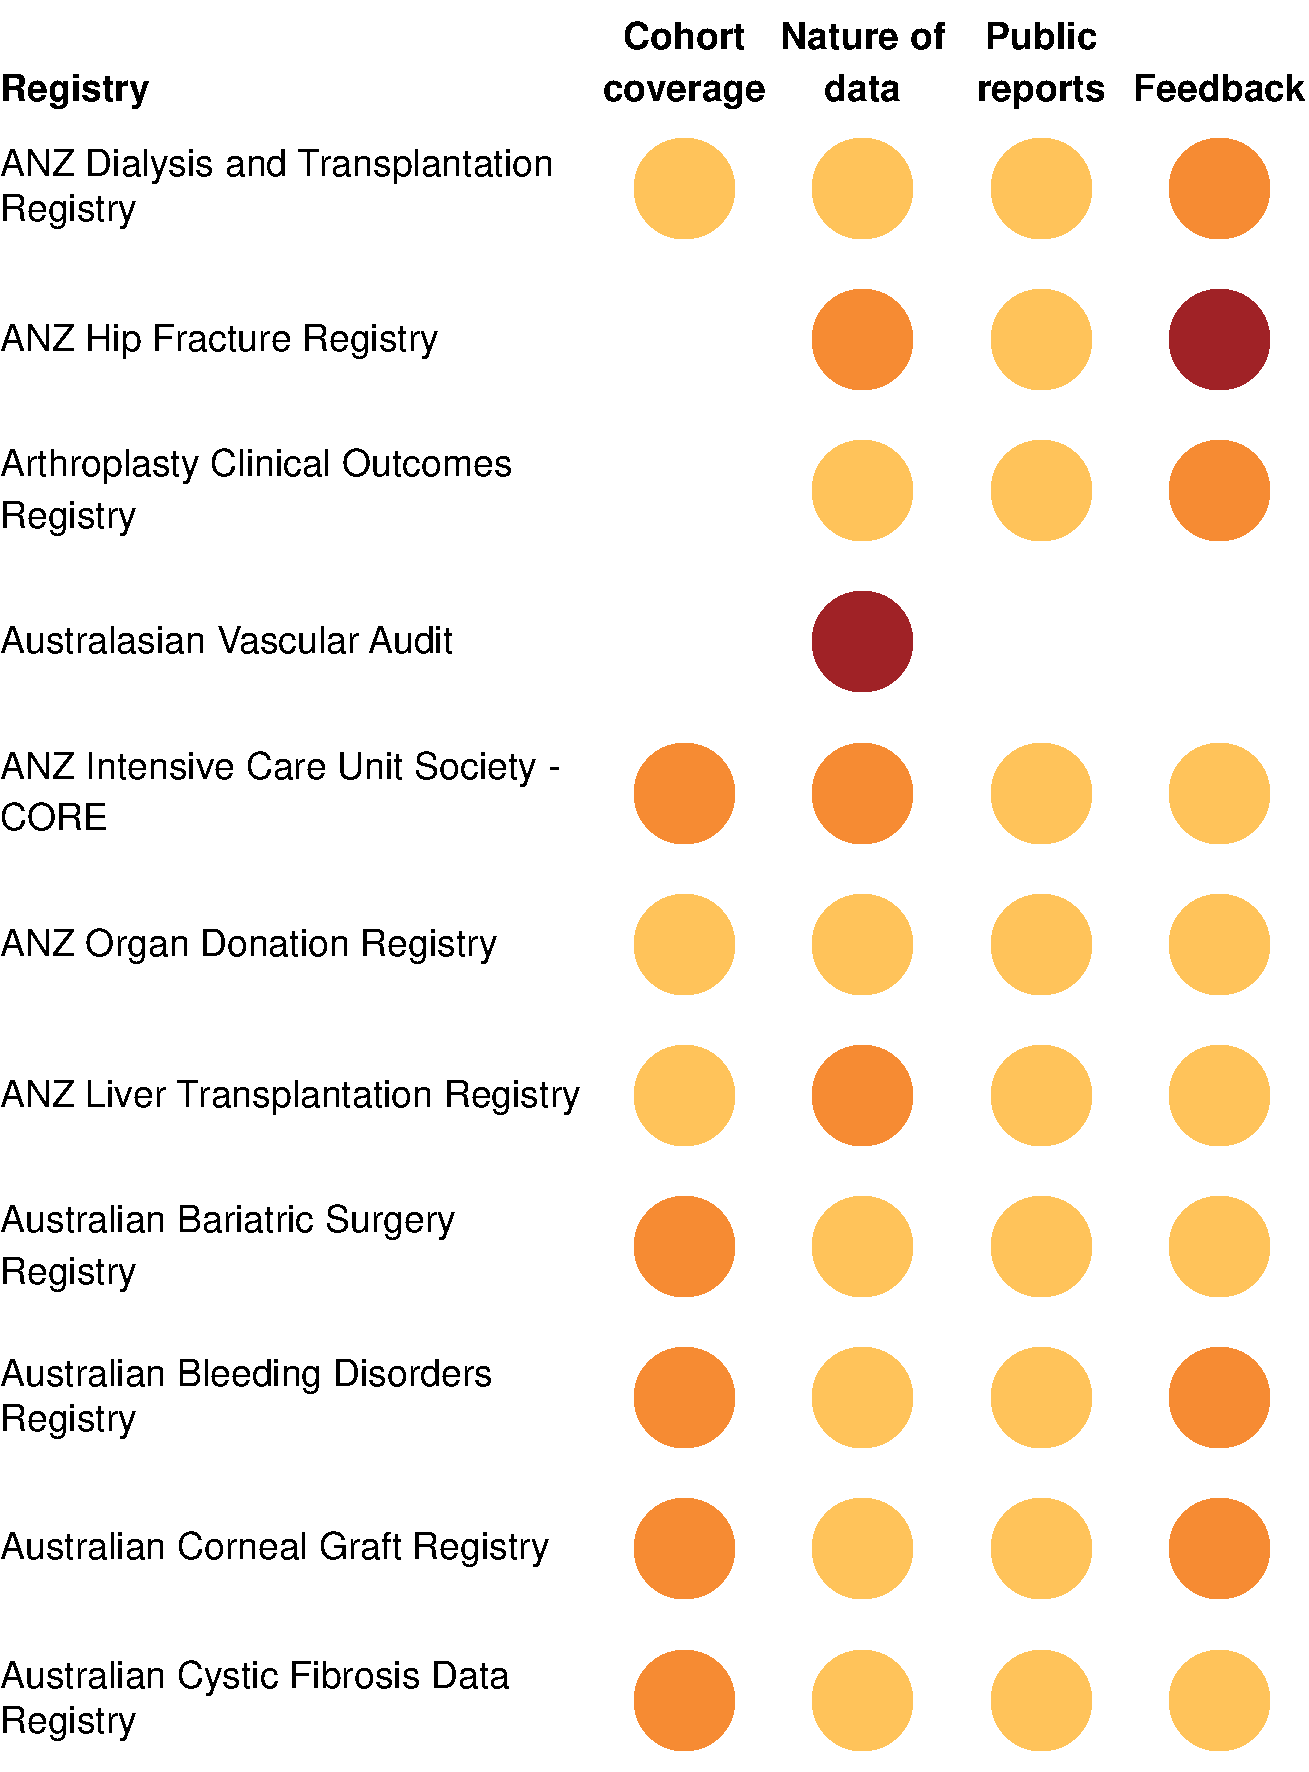
\includegraphics[page=1]{atlas/Registry_graphs.pdf}
\end{figure}

\begin{figure}
\includegraphics[page=2]{atlas/Registry_graphs.pdf}
\end{figure}

\begin{figure}
\includegraphics[page=3]{atlas/Registry_graphs.pdf}
\end{figure}

\begin{figure}
\includegraphics[page=4]{atlas/Registry_graphs.pdf}
\end{figure}

\printbibliography


\end{document}
